%\noindent
\justifying
\setlength{\parskip}{1em}

In this chapter, the methodology of our image-to-image translation application explained in depth. In Section \ref{ProposedApproach}, the proposed approach is pictorially described and theoretically explained. In Section \ref{CycleConsistentAdversarialNetworks}, the mathematics behind \ac{CycleGAN} is discussed thoroughly along with loss functions and objective functions. Also, the algorithm of the \ac{CycleGAN} described in Section \ref{CycleGANAlgorithm}.

\section{Proposed Approach}\label{ProposedApproach}


\begin{figure}[H]
        \begin{center}
    	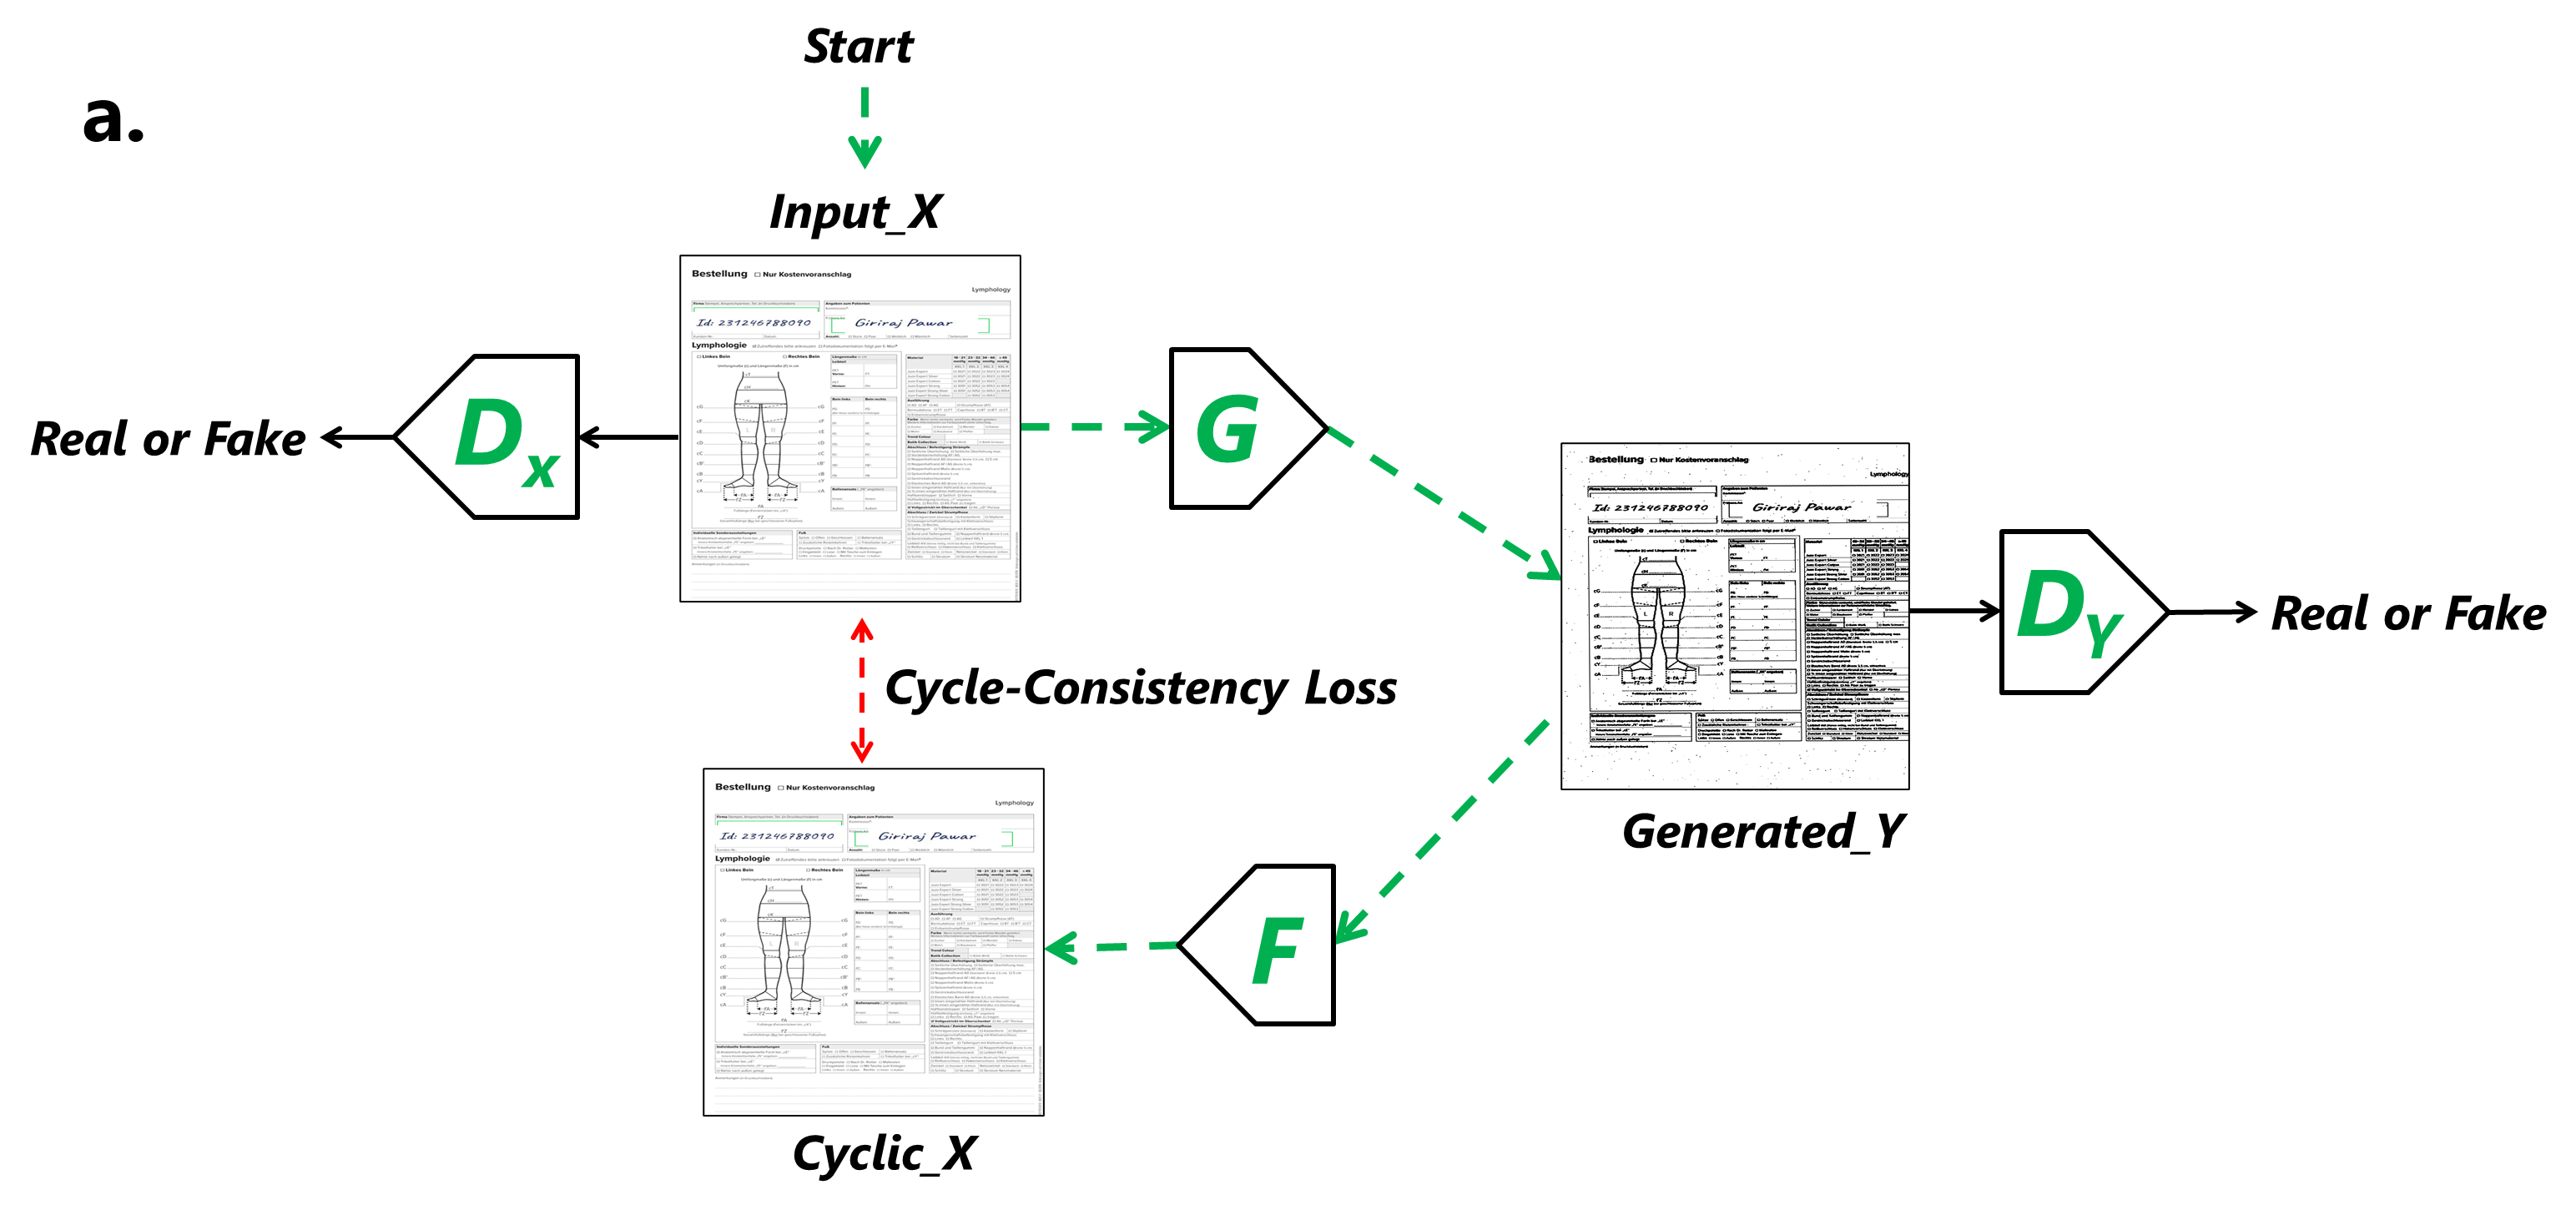
\includegraphics[scale=0.20]{images/Methodology/Gxy.png}
	    \caption[]{}
	    \label{fig:Gxy}
	    \end{center}
\end{figure}



\begin{figure}[H]
        \begin{center}
    	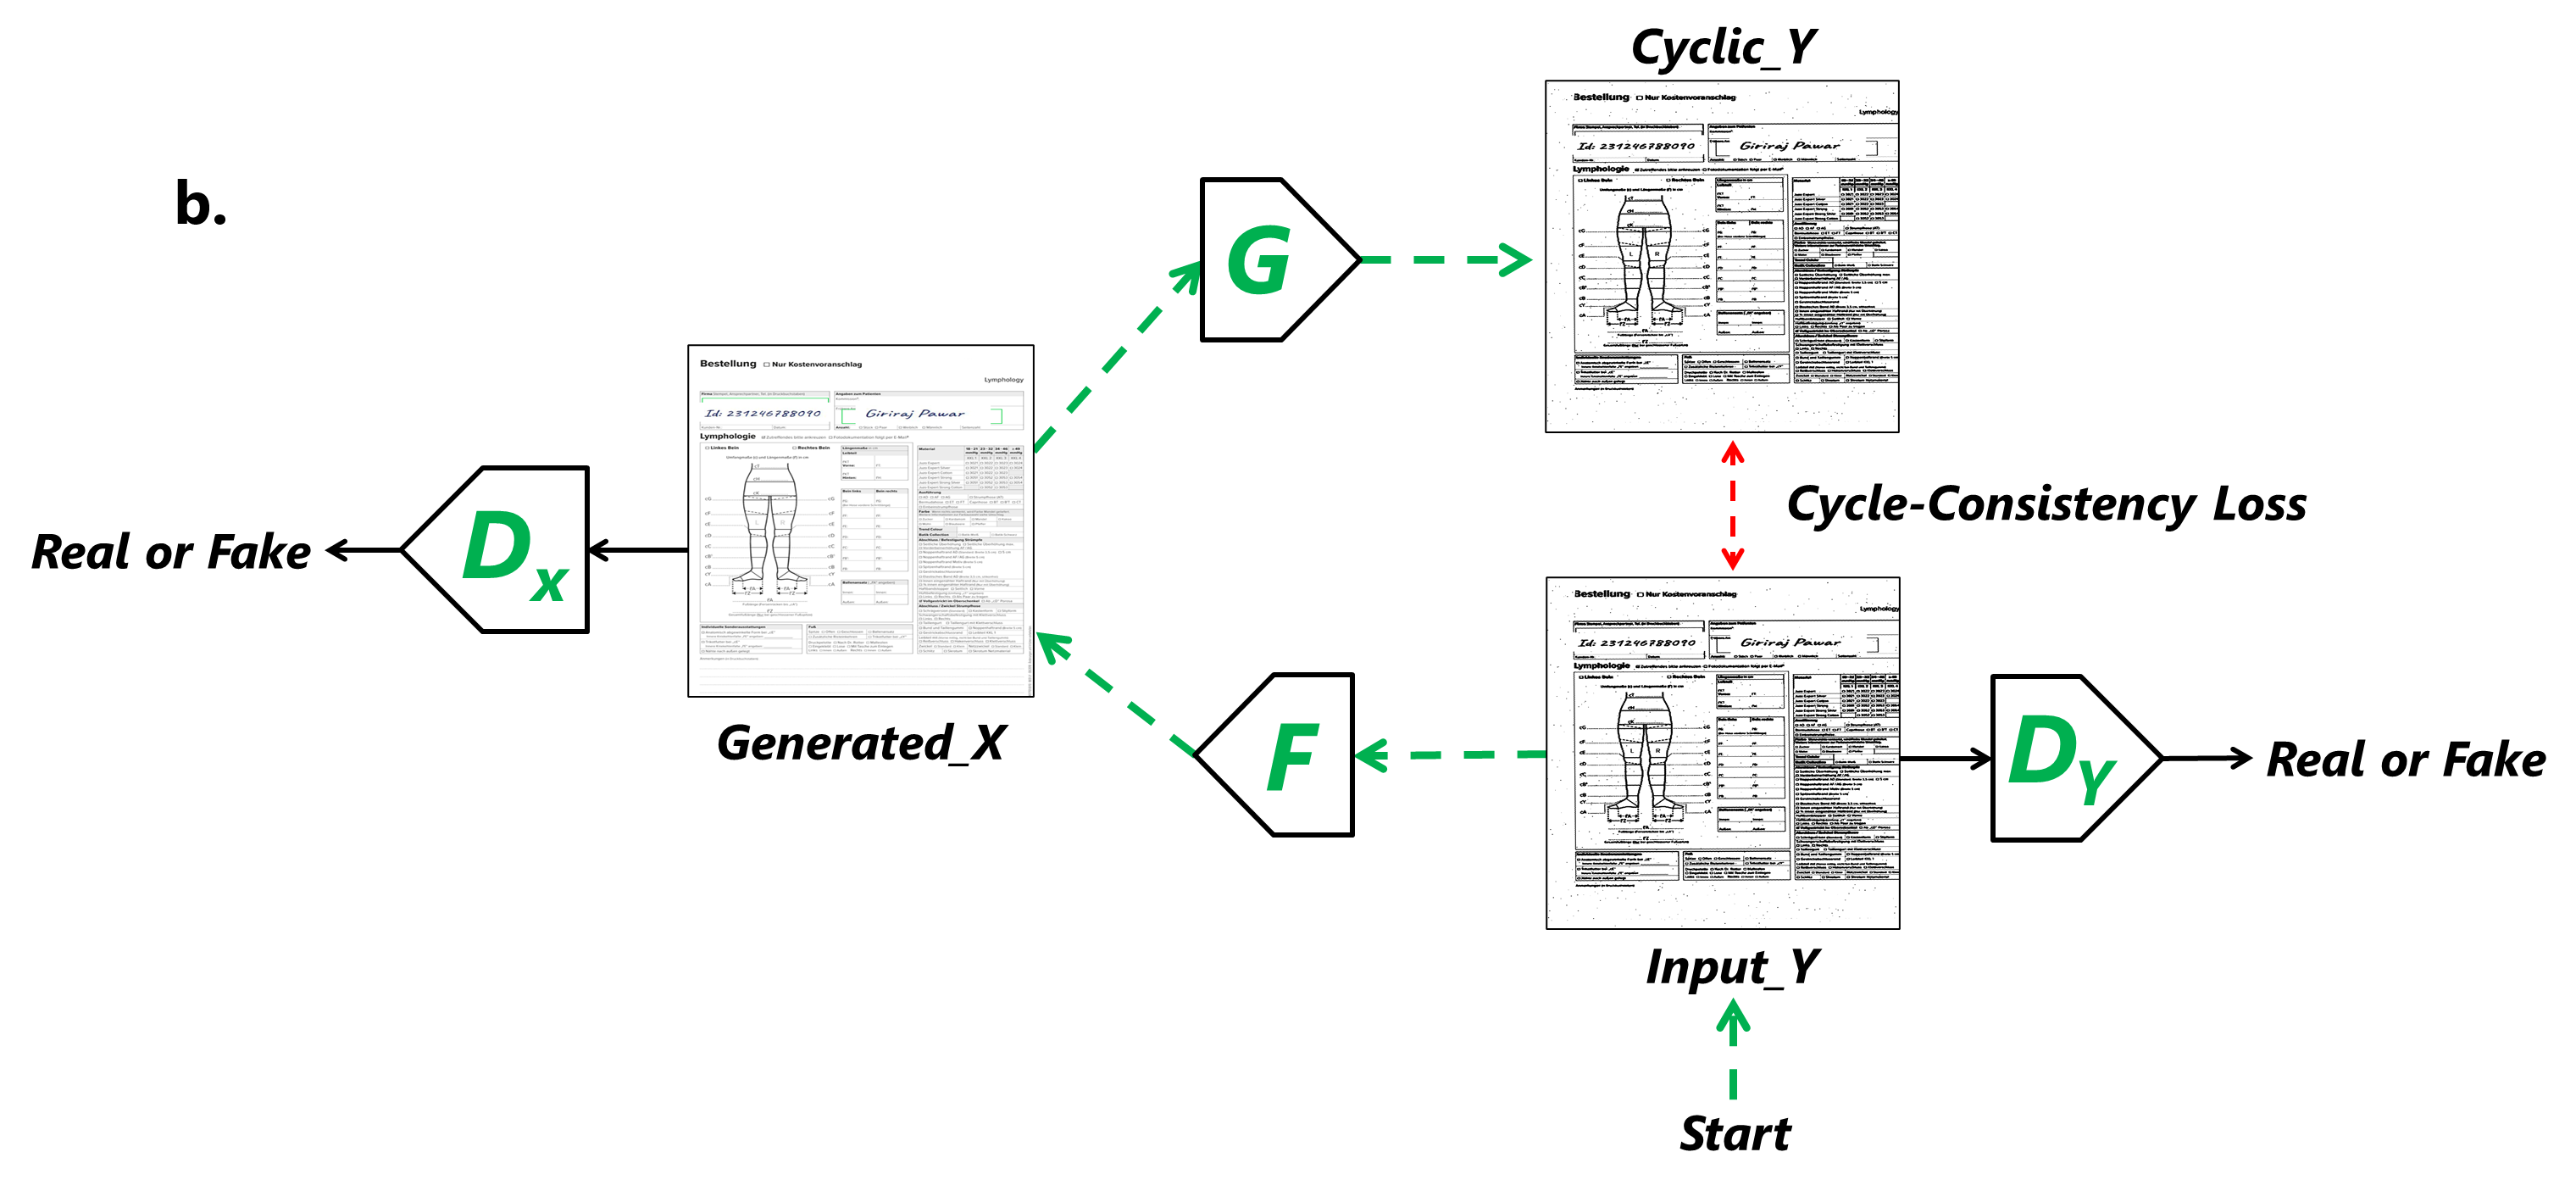
\includegraphics[scale=0.20]{images/Methodology/Fyx.png}
	    \caption[]{}
	    \label{fig:Fyx}
	    \end{center}
\end{figure}


\section{Cycle-Consistent Adversarial Networks}\label{CycleConsistentAdversarialNetworks}


\subsection{Formulation}


The aim is to learn mapping functions between two domains $X$ and $Y$. $X$ is the source domain and $Y$ is the target domain. The domain $X$ represents synthetic data distribution and domain $Y$ represents real data distribution. The synthetic data distribution is represented by synthetic document images created using empty form templates and handwritten crops. The real data distribution is represented by the real document images. For a given training samples $\{x_i\}_{i=1}^{N}$ where $x_i \in X$ and $\{y_j\}_{j=1}^{M}$ where $y_j \in Y$. The synthetic data distribution represented as $x \sim p_{data}(x)$ and real data distribution represented as $y \sim p_{data}(y)$. The model includes two mappings functions $G : X \rightarrow Y$ and $F : Y \rightarrow X$ as illustrated in figure \ref{fig:CycleGAN}, they are the generators. Along with generators, two adversarial discriminators $D_X$ and $D_Y$ are introduced. $D_X$ aims to distinguish between images $\{x\}$ and translated images $\{F(y)\}$. In the same way, $D_Y$ aims to discriminate between $\{y\}$ and $\{G(x)\}$.  The final objective function contains three loss functions. first, least-square loss\cite{mao2017squares} is used for matching the distribution of generated images to the data distribution in the target domain. The general \acp{GAN} uses sigmoid cross-entropy loss function to optimize generator and discriminator. In our thesis generators and discriminators used in \ac{CycleGAN} are optimized using least-square loss\cite{mao2017squares} which is opted from \acp{LSGAN}. Second, The cycle consistency loss to prevent the learned mappings functions $G$ and $F$ from contradicting each other\cite{zhu2020unpaired}. The third is identity mapping loss to preserve the color of the input images\cite{zhu2020unpaired}.


\subsection{Least-Square Loss}


In \acp{GAN} the discriminator is a binary classifier that adopts the sigmoid cross-entropy loss function. As stated in Section \ref{rwdiscussion}, while updating the generator, the sigmoid cross-entropy loss function causes the vanishing gradients problem for the samples that are on the correct side of the decision boundary but are still far from the real data.  Also, the sigmoid cross-entropy loss function causes difficulty to stabilize the model training procedure\cite{mao2017squares}. First, $\mathcal{L}_{GAN}$ (equation \ref{ganObjectiveFunction}), the negative log-likelihood objective replaced by a least-squares loss functions\cite{mao2017squares}. The least-squares loss is more stable during training and generates higher quality results\cite{mao2017squares}. It is used to optimize the generator and discriminator adversarially. In the below equations, we have used the $a$,$b$, and $c$ for the coding scheme for the equations of the discriminator. Where $a$ and $b$ are the labels for fake data and real data, respectively. $c$ denotes the value that G wants D to believe for fake data. Basically, $a = 0$, $b = 1$, and $c = 1$. That means fake data is represented by $0$, and real data is represented by $1$. Then the modified objective functions using least-squares loss can be defined as follows:



    \begin{equation}\label{lsgan1}
        \underset{D}{\min}\ \mathcal{L}_{LSGAN}(D_Y) = \frac{1}{2}\ \mathbb{E}_{y \sim p_{data}(y)}\ [(D(y) - b)^2] + 
        \frac{1}{2}\ \mathbb{E}_{x \sim p_{data}(x)}\ [(D(G(x)) - a)^2]
    \end{equation}
    
    \begin{equation}\label{lsgan2}
        \underset{G}{\min}\ \mathcal{L}_{LSGAN}(G) = \mathbb{E}_{x \sim p_{data}(x)}\ [(D(G(x)) - c)^2]
    \end{equation}
    
    \begin{equation}\label{lsgan3}
    \mathcal{L}_{LSGAN}(G, D_Y, X, Y) =  \underset{D}{\min}\ \mathcal{L}_{LSGAN}(D_Y) + \underset{G}{\min}\ \mathcal{L}_{LSGAN}(G)
    \end{equation}
    
    \begin{equation}\label{lsgan4}
        \underset{D}{\min}\ \mathcal{L}_{LSGAN}(D_X) = \frac{1}{2}\ \mathbb{E}_{x \sim p_{data}(x)}\ [(D(x) - b)^2] + 
        \frac{1}{2}\ \mathbb{E}_{y \sim p_{data}(y)}\ [(D(F(y)) - a)^2]
    \end{equation}
    
    \begin{equation}\label{lsgan5}        
        \underset{G}{\min}\ \mathcal{L}_{LSGAN}(F) = \mathbb{E}_{y \sim p_{data}(y)}\ [(D(F(y)) - c)^2]
    \end{equation}
    
    
    \begin{equation}\label{lsgan6}        
        \mathcal{L}_{LSGAN}(F, D_X, Y, X) = \underset{D}{\min}\ \mathcal{L}_{LSGAN}(D_X) + \underset{G}{\min}\ \mathcal{L}_{LSGAN}(F)
    \end{equation}
    






\subsection{Cycle Consistency Loss}\label{CycleConsistencyLoss}

Adversarial training can, in theory, learn mappings $G$ and $F$ that produce outputs identically distributed as target domains $Y$ and $X$ respectively. However, with large enough capacity, a network can map the same set of input images to any random permutation of images in the target domain, where any of the learned mappings can induce an output distribution that matches the target distribution. Thus, adversarial losses alone cannot guarantee that the learned function can map an individual input $x_i$ to a desired output $y_i$. To further reduce the space of possible mapping functions, we argue that the learned mapping functions should be cycle-consistent: as shown in Figure \ref{fig:CycleGAN} (b), for each image $x$ from domain $X$, the image translation cycle should be able to bring $x$ back to the original image, i.e., $x \rightarrow G(x) \rightarrow F(G(x)) \approx x$. We call this forward cycle consistency. Similarly, as illustrated in Figure \ref{fig:CycleGAN} (c), for each image $y$ from domain $Y$, $G$ and $F$ should also satisfy backward cycle consistency: $y \rightarrow F(y) \rightarrow G(F(y)) \approx y$. We incentivize this behavior using a cycle consistency loss: 

\begin{equation}\label{CycleConsistencyLossEquation}
    \mathcal{L}_{cyc}(G, F) = \mathbb{E}_{x \sim p_{data}(x)}[\|F(G(x)) - x\|_1] + \mathbb{E}_{y \sim p_{data}(y)}[\|G(F(y)) - y\|_1].
    \end{equation}

\begin{figure}[H]
	    \begin{center} 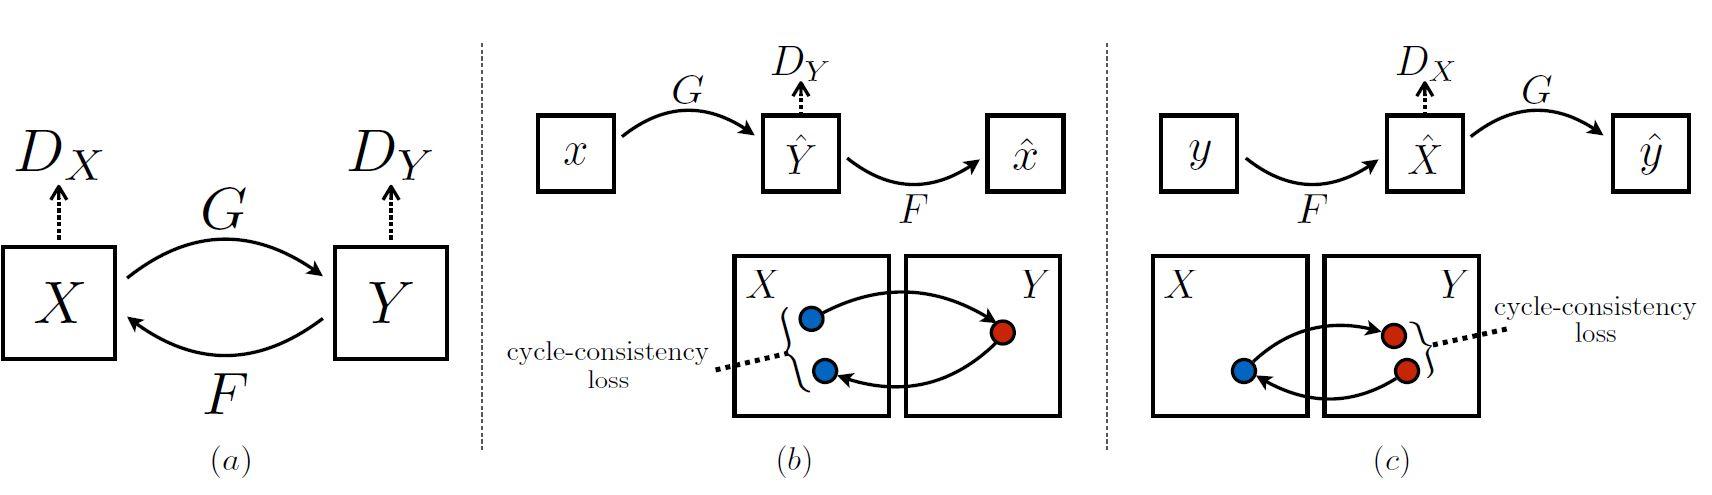
\includegraphics[scale=0.5]{images/CycleGAN.jpg}
	    \caption[CycleGAN Model Mapping Functions.]{(a) CycleGAN model contains two mapping functions $G : X \rightarrow Y$ and $F : Y \rightarrow X$, and associated adversarial discriminators $D_Y$ and $D_X$. $D_Y$ encourages $G$ to translate $X$ into outputs indistinguishable from domain $Y$, and vice versa for $D_X$ and $F$. To further regularize the mappings, we introduce two cycle consistency losses that capture the intuition that if we translate from one domain to the other and back again we should arrive at where we started: (b) forward cycle-consistency loss: $x \rightarrow G(x) \rightarrow F(G(x)) \approx x$, and (c) backward cycle-consistency loss: $y \rightarrow F(y) \rightarrow G(F(y)) \approx y$ ~\cite{zhu2020unpaired}.}
	    \label{fig:CycleGAN}
	    \end{center}
\end{figure}

\subsection{Identity Mapping Loss}

It is helpful to introduce an additional loss to encourage the mapping to preserve color composition between the input and output. In particular, we adopt the technique of \cite{taigman2016unsupervised} and regularize the generator to be near an identity mapping when real samples of the target domain are provided as the input to the generator:

\begin{equation}\label{IdentityMappingLoss}
    \mathcal{L}_{identity}(G, F) = \mathbb{E}_{y \sim p_{data}(y)}[\|(F(y) - y\|_1] + \mathbb{E}_{x \sim p_{data}(x)}[\|G(x) - x\|_1]. 
    \end{equation}

\subsection{Full Objective}

The full objective is:
\begin{equation}\label{FullObjective}
\begin{aligned}
    \mathcal{L}(G, F, D_X, D_Y) =  \mathcal{L}_{LSGAN}(G, D_Y, X, Y)\ +\ \mathcal{L}_{LSGAN}(F, D_X, Y, X)\ +\ \\
    \lambda_{identity}\ \mathcal{L}_{identity}(G, F)\ +\ \lambda_{cyc}\ \mathcal{L}_{cyc}(G, F),
\end{aligned}
\end{equation}
    
where $\lambda_{cyc}$ and $\lambda_{identity}$ control the relative importance of the two objectives.




\section{Algorithm}\label{CycleGANAlgorithm}


%%%%%%%%%%%%%%%%%%%%%%%%%%%%%%%%%%%%%%%%%%%%%%%%%%%%%%%%%%%%%%%%%%%%%%%%%%%%%%%%%%%%%%%%%%%%%%%%%%%%%%%%%%%%%%%%%5


%The aim is to learn mapping functions between two domains $X$ and $Y$. The Domain $X$ represents synthetic document images distribution and domain $Y$ represents real document images distribution. Given training samples $\{x_i\}_{i=1}^{N}$ where $x_i \in X$ and  $\{y_j\}_{j=1}^{M}$ where $y_j \in Y$. We denote the data distribution $x \sim p_{data}(x)$  and $y \sim p_{data}(y)$.

\begin{comment}
\subsection{Adversarial Loss}
We apply adversarial losses \cite{goodfellow2014generative} to both mapping functions. For the mapping function $G : X \rightarrow Y$  and its discriminator $D_Y$ , we express the objective as:

    \begin{equation}\label{AdversarialLoss}
    \mathcal{L}_{GAN}(G, D_Y, X, Y) = \mathbb{E}_{y \sim p_{data}(y)} [\log D_Y(y)] + \mathbb{E}_{x \sim p_{data}(x)}[\log (1 - D_Y(G(x)))],
    \end{equation}
    
where $G$ tries to generate images $G(x)$ that look similar to images from domain $Y$ , while $D_Y$ aims to distinguish between translated samples $G(x)$ and real samples $y$. $G$ aims to minimize this objective against an adversary $D$ that tries
to maximize it, i.e., $\min_{G} \max_{D_Y} \mathcal{L}_{GAN}(G, D_Y, X, Y)$. We introduce a similar adversarial loss for the mapping function $F : Y \rightarrow X$ and its discriminator $D_X$ as well: i.e., $\min_{F} \max_{D_X} \mathcal{L}_{GAN}(F, D_X, Y, X)$.

\end{comment}




\begin{comment}
We aim to solve:
\begin{equation}\label{FullObjectiveAimToSolve}
    G^*, F^* = \arg\underset{G, F}{\min}\underset{D_X, D_Y}{\min} \mathcal{L}(G, F, D_X, D_Y)
    \end{equation}
\end{comment}






